Deployment diagram mô tả kiến trúc triển khai (deployment architecture) của hệ thống Social Commerce, bao gồm các thành phần phần cứng, phần mềm, môi trường triển khai và các kết nối giữa chúng. Diagram này giúp hiểu rõ cách hệ thống được triển khai trên môi trường production và cách các thành phần tương tác với nhau.

\subsection{Tổng quan kiến trúc triển khai}

\ref{fig:deployment-diagram} mô tả kiến trúc triển khai tổng thể của hệ thống, bao gồm các layers chính: Client Layer, CDN Layer, Application Server, Database và External Services.

\begin{figure}[htbp]
    \centering
    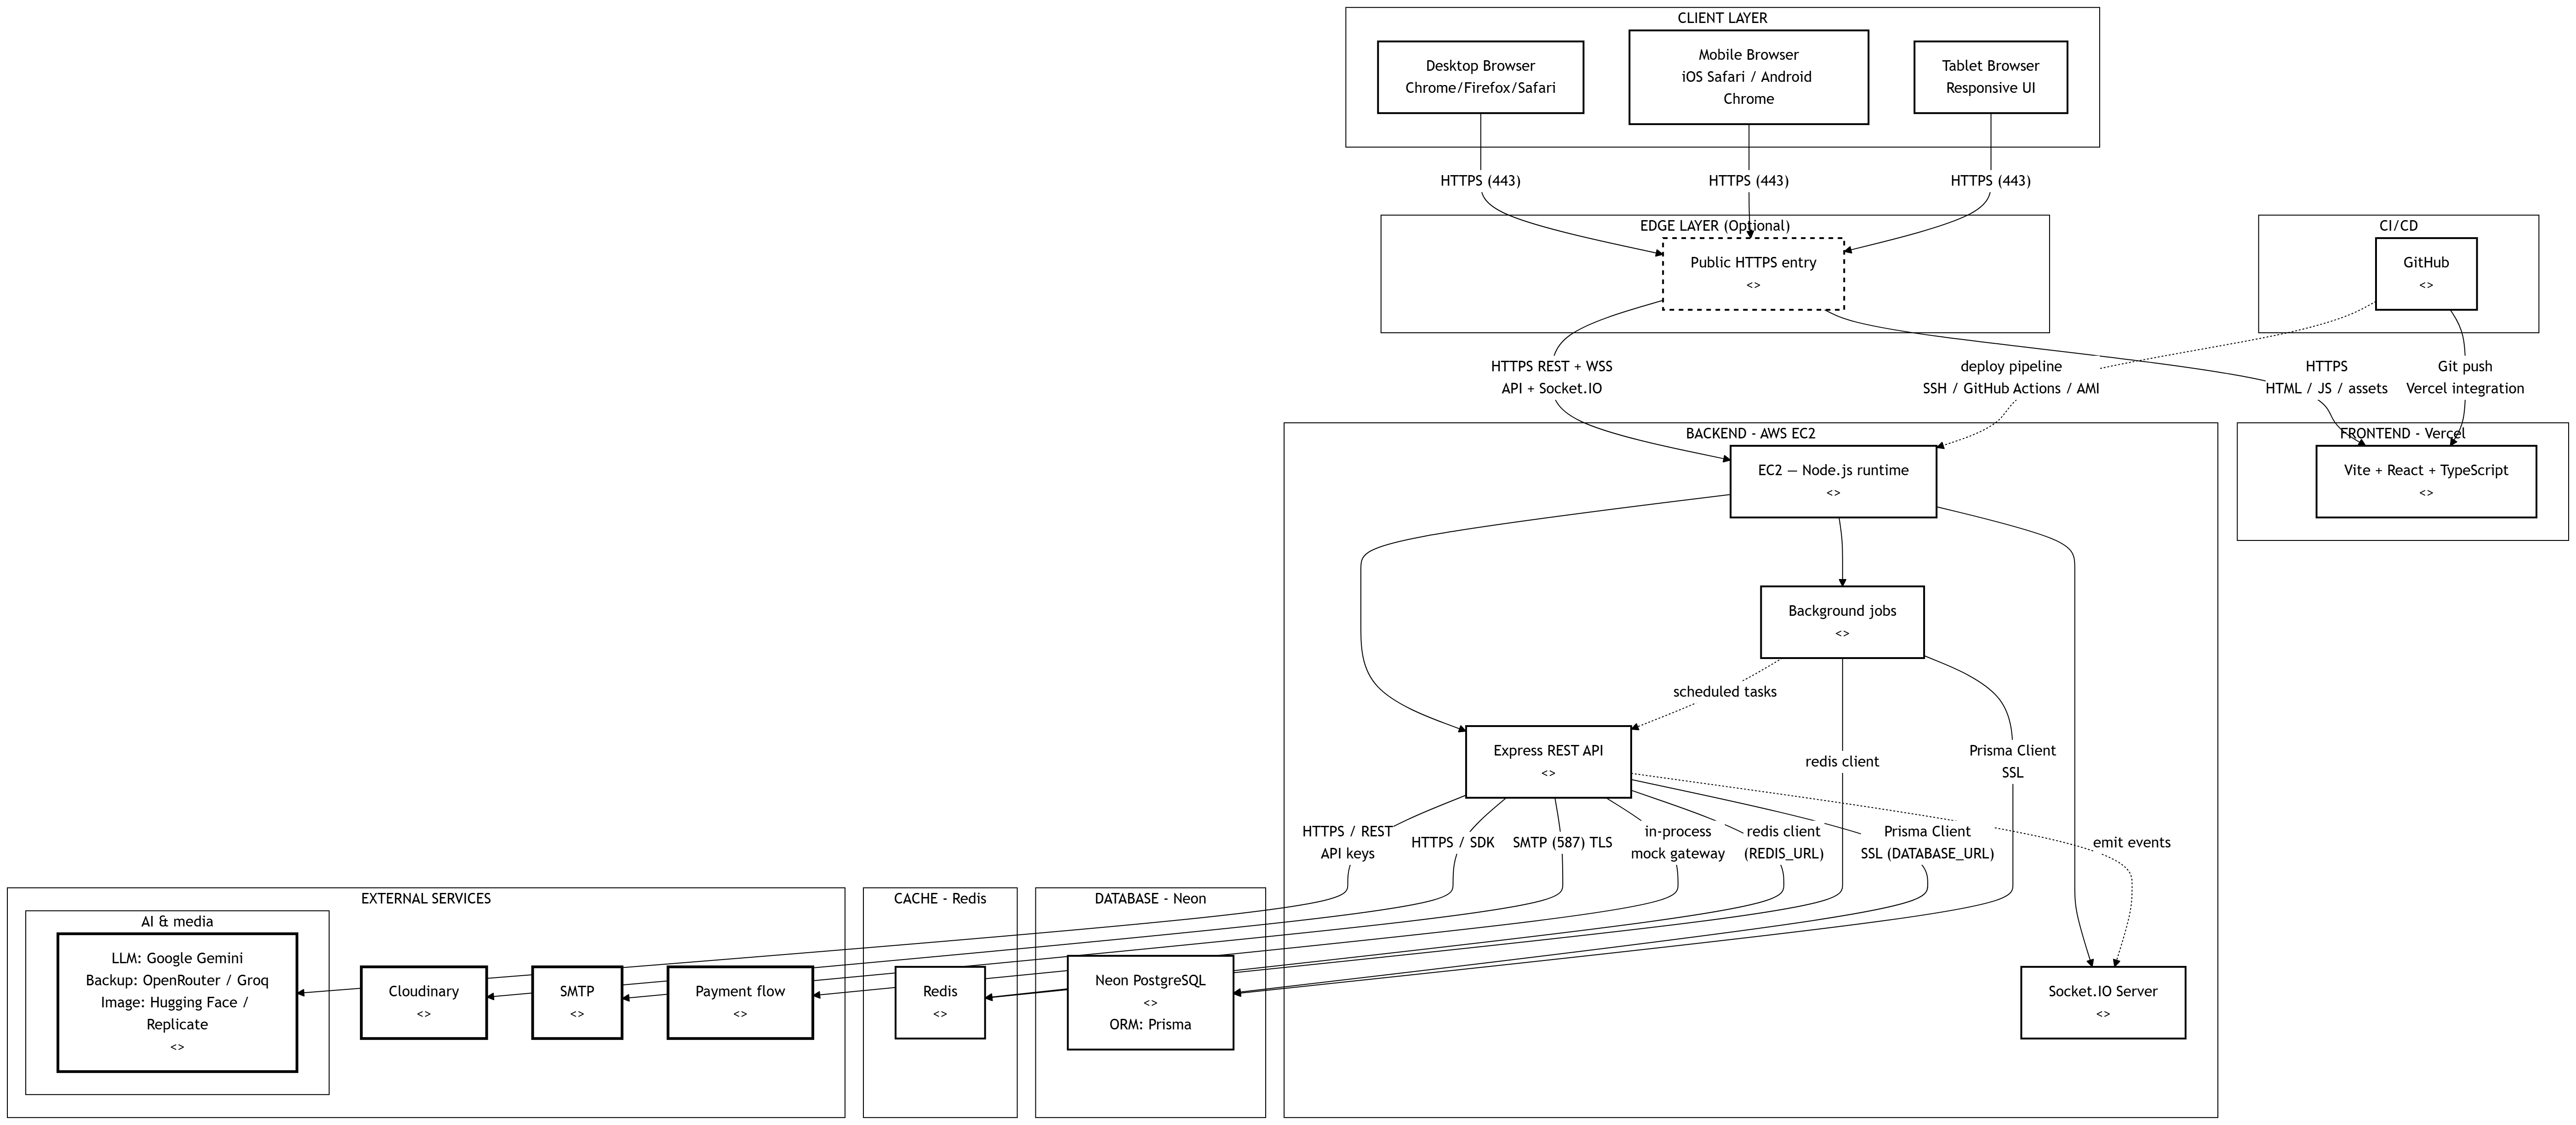
\includegraphics[width=\textwidth]{Images/Deployment Diagram.png}
    \caption{Deployment Diagram - Kiến trúc triển khai hệ thống}
    \label{fig:deployment-diagram}
\end{figure}

\subsection{Các thành phần chính}

\subsubsection{Client Layer}

\textbf{Client Layer} bao gồm các thiết bị và trình duyệt mà người dùng sử dụng để truy cập hệ thống:

\begin{itemize}
    \item \textbf{Desktop Browser}: Chrome, Firefox, Safari trên máy tính
    \item \textbf{Mobile Browser}: iOS Safari, Android Chrome trên điện thoại di động
    \item \textbf{Tablet Browser}: Giao diện responsive trên máy tính bảng
\end{itemize}

Tất cả các client kết nối đến hệ thống thông qua giao thức \textbf{HTTPS (port 443)} cho các request thông thường và \textbf{WebSocket Secure (WSS)} cho các tính năng real-time như thông báo và chat.

\subsubsection{CDN Layer (Optional)}

\textbf{Cloudflare CDN} là tầng tùy chọn được sử dụng để:

\begin{itemize}
    \item \textbf{Caching}: Lưu cache các static assets (HTML, CSS, JavaScript, images) để tăng tốc độ tải trang
    \item \textbf{DDoS Protection}: Bảo vệ hệ thống khỏi các cuộc tấn công DDoS
    \item \textbf{SSL/TLS Termination}: Xử lý chứng chỉ SSL/TLS, giảm tải cho application server
\end{itemize}

Khi CDN được triển khai, các static files sẽ được phục vụ từ CDN (cache hit), trong khi các request động sẽ được chuyển tiếp đến application server (cache miss). WebSocket connections có thể bypass CDN để kết nối trực tiếp với application server để đảm bảo độ trễ thấp.

\subsubsection{Application Server}

Hệ thống được triển khai trên \textbf{Render.com}, một platform-as-a-service (PaaS) cloud, với các thành phần sau:

\paragraph{Node.js Runtime} 
Môi trường thực thi sử dụng \textbf{Node.js version >= 18.0.0}, cung cấp nền tảng để chạy ứng dụng backend.

\paragraph{React Frontend}
Frontend được build bằng \textbf{Vite} và được deploy dưới dạng static files. Trong production, Express server phục vụ các static files này từ thư mục \texttt{frontend/dist/}, bao gồm:
\begin{itemize}
    \item HTML files
    \item JavaScript bundles
    \item CSS stylesheets
    \item Assets (images, fonts, etc.)
\end{itemize}

\paragraph{Express API Server}
Backend được xây dựng bằng \textbf{Express.js framework}, chịu trách nhiệm:
\begin{itemize}
    \item Xử lý các REST API endpoints
    \item Áp dụng middleware stack (authentication, validation, rate limiting, error handling)
    \item Thực thi business logic thông qua controllers
    \item Tích hợp với các external services
\end{itemize}

\paragraph{Socket.IO Server}
\textbf{Socket.IO server} được tích hợp vào cùng application server, cung cấp:
\begin{itemize}
    \item \textbf{WebSocket connections}: Kết nối real-time hai chiều với clients
    \item \textbf{Real-time events}: Gửi và nhận events real-time
    \item \textbf{Chat rooms}: Quản lý các phòng chat
    \item \textbf{Push Notifications}: Gửi thông báo tức thì đến clients
    \item \textbf{Live Updates}: Cập nhật trạng thái real-time (order status, notifications, etc.)
\end{itemize}

Socket.IO server tương tác với Express server để emit events khi có các thay đổi trong hệ thống (ví dụ: khi có đơn hàng mới, notification mới).

\paragraph{Background Jobs}
Hệ thống sử dụng \textbf{node-cron} để chạy các background jobs theo lịch:
\begin{itemize}
    \item \textbf{Auto-publish scheduled posts}: Tự động publish các bài viết đã được lên lịch
    \item \textbf{Cleanup old notifications}: Xóa các thông báo cũ
    \item \textbf{Reset monthly AI usage}: Reset số lần sử dụng AI theo tháng
    \item \textbf{Clean expired content requests}: Xóa các yêu cầu tạo nội dung AI đã hết hạn
\end{itemize}

Các cron jobs được chạy in-process trong cùng application server, không cần infrastructure riêng biệt.

\subsubsection{Database - PostgreSQL}

Hệ thống sử dụng \textbf{PostgreSQL} làm database chính:

\begin{itemize}
    \item \textbf{Managed Database}: Database được quản lý bởi Render.com hoặc cloud provider khác
    \item \textbf{ORM: Sequelize}: Sử dụng Sequelize ORM để tương tác với database, cung cấp abstraction layer và hỗ trợ migrations
    \item \textbf{SSL/TLS Connection}: Tất cả các kết nối đến database đều được mã hóa bằng SSL/TLS để đảm bảo bảo mật
\end{itemize}

Express server và cron jobs đều kết nối đến PostgreSQL thông qua Sequelize ORM để thực hiện các thao tác CRUD và query dữ liệu.

\subsubsection{External Services}

Hệ thống tích hợp với các external services để cung cấp các tính năng bổ sung:

\paragraph{AI Services}
\textbf{Google Gemini API và Google Veo 2} được sử dụng để:
\begin{itemize}
    \item Tạo bài viết từ mô tả, ý tưởng và hình ảnh sản phẩm (Generate Text)
    \item Tạo đồng thời bài viết và hình ảnh từ mô tả, ý tưởng và hình ảnh đầu vào (Generate Image + Text)
    \item Tạo video ngắn kèm tối đa 3 hình ảnh và bài viết từ mô tả, ý tưởng và hình ảnh đầu vào (Generate Video + Images + Text)
\end{itemize}

Kết nối đến Gemini API và Veo 2 sử dụng HTTPS/REST với API Key authentication. Hệ thống quản lý usage limit cho từng người dùng để kiểm soát chi phí và tài nguyên.

\paragraph{File Storage}
\textbf{Cloudinary} được sử dụng để:
\begin{itemize}
    \item Lưu trữ và quản lý hình ảnh, video
    \item Tối ưu hóa hình ảnh (resize, compress, format conversion)
    \item Cung cấp CDN global để phân phối assets nhanh chóng
\end{itemize}

Kết nối đến Cloudinary sử dụng HTTPS/REST API để upload và quản lý files.

\paragraph{Email Service}
\textbf{Gmail SMTP} được sử dụng để:
\begin{itemize}
    \item Gửi email thông báo đến người dùng
    \item Gửi email xác nhận đơn đăng ký seller
    \item Gửi email thông báo về đơn hàng, reviews, etc.
\end{itemize}

Kết nối sử dụng SMTP protocol (port 587) với TLS encryption, thông qua Nodemailer library.

\paragraph{Payment Simulator}
\textbf{Payment Simulator} là một mock service chạy local trong application server:
\begin{itemize}
    \item Mô phỏng quá trình thanh toán (success/failure)
    \item Chỉ sử dụng cho development và testing
    \item Không có kết nối mạng ngoài, không xử lý tiền thật
\end{itemize}

\subsubsection{CI/CD Pipeline}

\textbf{GitHub} được sử dụng làm repository để:
\begin{itemize}
    \item Lưu trữ source code
    \item Version control
    \item Quản lý pull requests và code reviews
\end{itemize}

\subsection{Đặc điểm kiến trúc}

\paragraph{Monolithic Deployment}
Hệ thống được triển khai dưới dạng monolithic architecture, tất cả các components (Frontend, Backend API, Socket.IO, Cron Jobs) chạy trong cùng một application server. Điều này đơn giản hóa việc triển khai và quản lý, phù hợp với quy mô hiện tại của dự án.

\paragraph{Server-Side Rendering Static Files}
Frontend React được build thành static files và được phục vụ bởi Express server. Điều này cho phép:
\begin{itemize}
    \item Single deployment cho cả frontend và backend
    \item Không cần CDN riêng cho static files (tùy chọn)
    \item Dễ dàng quản lý và deploy
\end{itemize}

\paragraph{Real-time Communication}
Socket.IO được tích hợp trực tiếp vào application server, cho phép real-time communication mà không cần infrastructure riêng biệt. Điều này đơn giản hóa kiến trúc nhưng có thể ảnh hưởng đến khả năng mở rộng (scalability) nếu số lượng WebSocket connections tăng cao.

\paragraph{External Service Integration}
Hệ thống tích hợp với các external services thông qua REST API và SMTP, giúp:
\begin{itemize}
    \item Giảm tải cho application server (file storage, email sending)
    \item Tận dụng các dịch vụ chuyên nghiệp (AI content generation, cloud storage)
    \item Dễ dàng thay thế hoặc bổ sung services khi cần
\end{itemize}

\paragraph{Bảo mật}
Tất cả các kết nối đều được mã hóa:
\begin{itemize}
    \item Client $\leftrightarrow$ Server: HTTPS/WSS (SSL/TLS)
    \item Application $\leftrightarrow$ Database: SSL/TLS connection
    \item Application $\leftrightarrow$ External Services: HTTPS (REST API) hoặc TLS (SMTP)
\end{itemize}

